\section{Debiasing Skin Lesion Datasets and Model. Not So Fast}\label{sec:debias-not-so-fast}
In their paper
''Debiasing Skin Lesion Datasets and Model. Not So Fast''
Bissoto, Alceu and Valle look into debiasing models trained on
skin lesion images \cite{debias-not-so-fast}.
They go through $7$ differenct artifacts in the images that could
be confunding elements, and try state of the art methods to
make them disregard the artifacts.
These include the rulers, that is the focus of this report.
The paper makes several claims about biases that occur in
skin lesion models.
Their focus is the removal of bias, but in that proces they
make claims about the model actually being biased.

\subsection{Arguments for the model being biased}
The researchers trained multiple different models to detect if the
images contained malignant or benign lesions.
Note that this classification is a simlified version of the classes
that is used in this report (see the severity column of Table \ref{table:ham10000}).
Just as in this report, the researchers also used the RESNET-18 architecture.
They then utilize that the architecture is setup in way where first a set of features
are extracted from the images using convolutional layers, and then fed into a fully connected layer. 
An outline of this is shown on Figure \ref{fig:resnet-outline}.
As shown in the figure, thwe convolutional layer exports a tensor.
This tensor can then be converted into a vector, which can be interpreted as a feature vector for the image.
Intuitively two images with \textit{similar} elements in the image should have a similar feature vector.
Utilizing this idea the researchers calculate these vectors for the entire test dataset.
The researchers then find that there is a small euclidean distance between the feature vectors of images
that have the same artifacts.
They show this by finding the nearest neighbors (with the distance measure between images being the euclidean distance between their feature vectors)
of different images artifact, and find that these neighbors often contain the same artifacts.
Their results are shown in Figure \ref{fig:not-so-fast-artifact-query}.


\begin{center}
    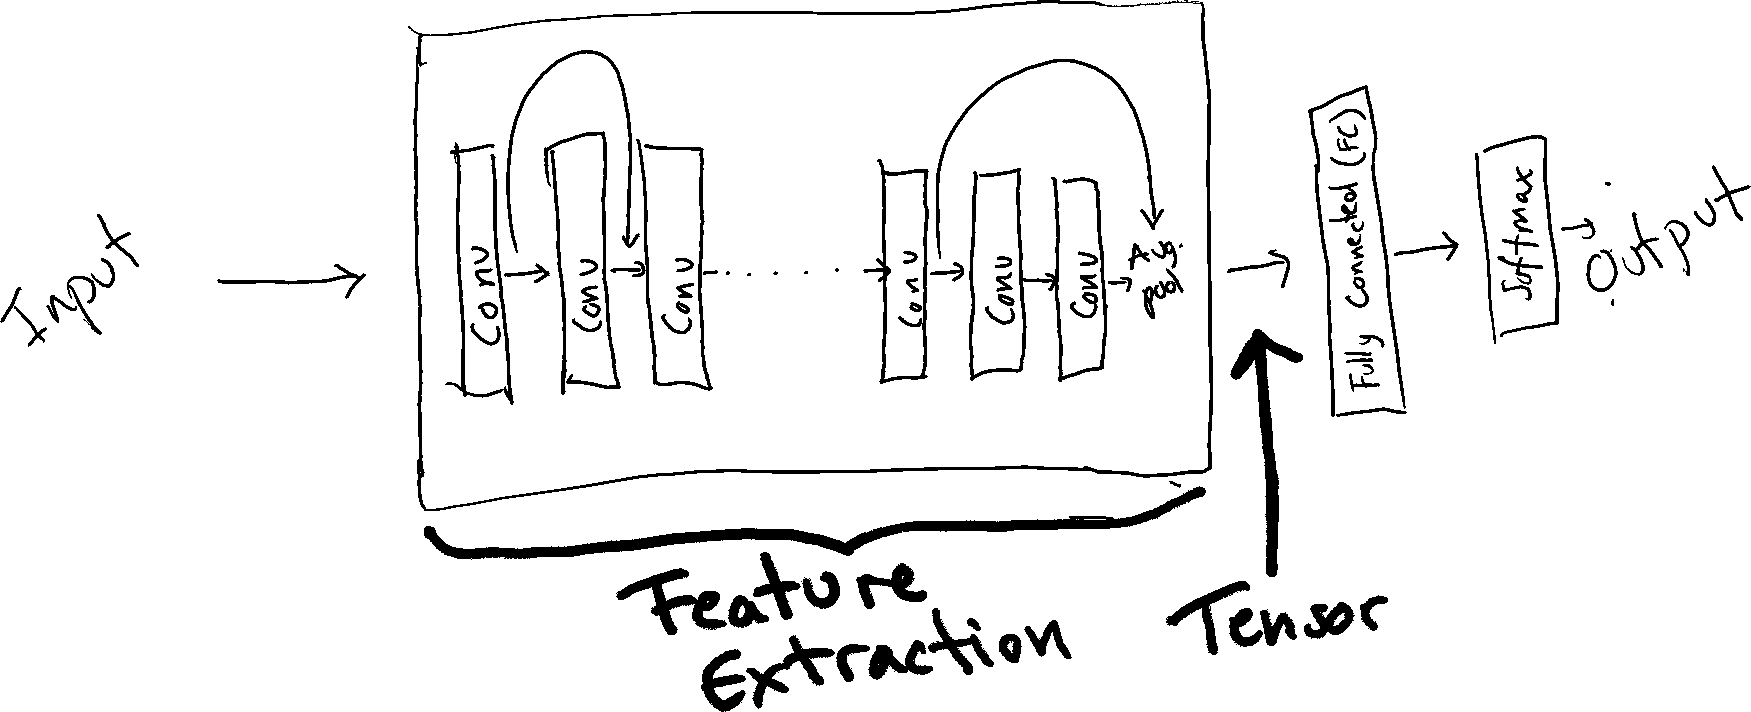
\includegraphics[width=0.9\textwidth]{images/resnet-outline.png}
    \captionof{figure}{A simplified view of the RESNET-18 architecture}
    \label{fig:resnet-outline}
\end{center}

\begin{center}
    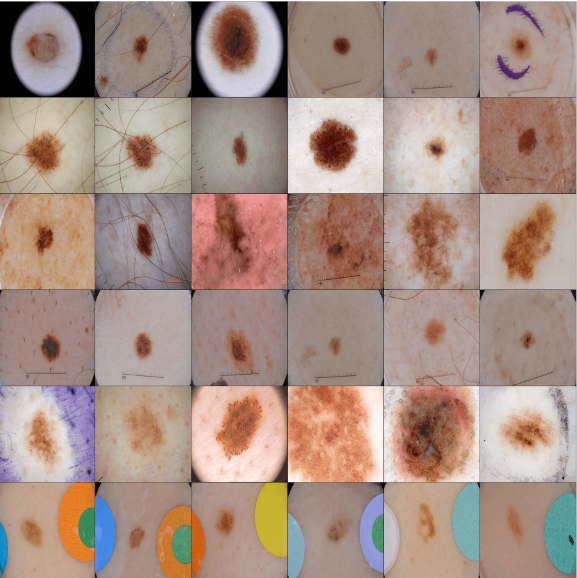
\includegraphics[width=0.4\textwidth]{images/not-so-fast-artifact-query.png}
    \captionof{figure}[Figure 4.a from \cite{debias-not-so-fast}]{
            Figure 4.a from \cite{debias-not-so-fast}, original description: \textit{Grid showing image similarity according to the features extracted by our classification model. The first column
            of each grid is the query, and the remaining columns are ranked according to euclidean distance of the images features.
            We selected queries carefully to show different artifacts.
            In sequence, dark corners, hair, gel border, ruler, ink markings and patches}}
    \label{fig:not-so-fast-artifact-query}
\end{center}

From the fact that the feature vectors of the images with the same artifacts are relatively small,
they conclude that the model is biased towards the artifacts - since the features it extracts seem to contain information about the artifacts.
The paper then goes on to examining how to mitigate these biases, but this is not relavant to this report.